\chapter{Introduction}
This Chapter briefly introduces the exercise and how we chose to approach it.

\section{Exercise Description}

The goal of this exercise, as described in the course compendium \cite{compendium}, is to implement a multi-cycle processor in VHDL, supporting a subset of the MIPS instruction set.
Some modules (data / instruction memory and \texttt{hostcomm}-communication) is handed out by the course staff.
A top level module (\texttt{MIPSSystem}) has also been provided, to facilitate testing on the FPGA.
The top level system architecture is illustrated in figure \ref{fig:sysarch}.


\begin{figure}[h!]
    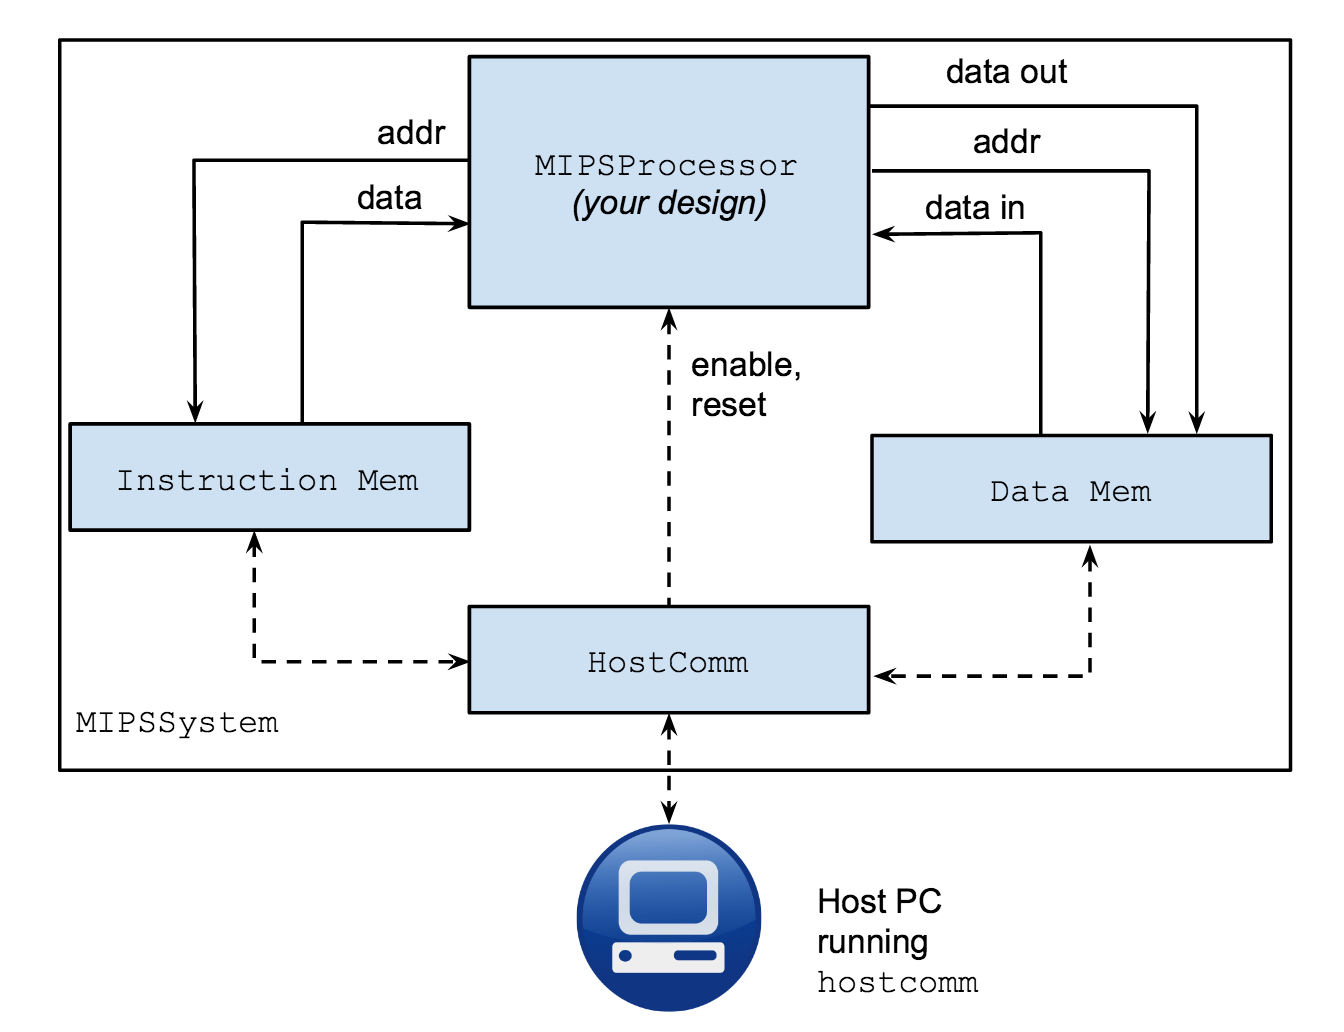
\includegraphics[width=\linewidth]{img/sysarch.png}
    \caption{The top-level architecture. Figure taken from the compendium. \cite[p. 48]{compendium}}
    \label{fig:sysarch}
\end{figure}

\newpage
Our job in this exercise is to implement the MIPSProcessor module in figure \ref{fig:sysarch} as a multi-cycle, MIPS-like processor.
The following categories of MIPS instructions are required to be implemented:

\begin{itemize}
    \item ALU operations - ADD, SUB, SLT, AND, OR
    \item Conditional branch - BEQ
    \item LOAD and STORE
    \item Load immediate - LDI
    \item Jump - JMP
\end{itemize}

\section{Approach}

We chose to start our work by sketching RTL designs based on the microarchitecture suggested by the course staff in the compendium \cite[p. 45]{compendium}.
Based on these sketches, we wrote VHDL to implement each of the following modules: Program counter, Register and ALU.
We also wrote testbenches for each of the modules, allowing us to test them independently from the system as a whole.
These components were then wired together in the MIPSProcessor module.
Signals going into and out of the MIPSProcessor were also routed to their appropriate submodules.
The final piece of the puzzle is the Control module, which we implemented based on figure 4.2 in the compendium \cite[p. 46]{compendium}.
